\section{Systematic uncertainties}
%%%%%%%%%%%%%%%%%%%%%%%%%%%%%%%%%%%%%%%%%%%%%%%%%%%%%%%%%%%%%%%%%%%%%%
\label{sec:Systematics}

Systematic uncertainties play an important role in this analysis where
no strong mass peak is expected due to the presence of undetected
neutrinos in the final state.  One of the most important sources of
systematic uncertainty is the normalization of the backgrounds that
are estimated on data control samples whenever is possible.
%%%Detailed numbers for all the nuisances and for all the samples 
%%%are reported in Appendix \ref{sec:nuisances}.

%-------------------------------------------------------------------------------
\subsection{Background normalization uncertainties}
%-------------------------------------------------------------------------------

The signal extraction is performed subtracting the estimated backgrounds to the event counts in data.
This uncertainty depends on the background: 
  \begin{itemize}
    \item {\bf\boldmath \ttbar and tW backgrounds:} 
      The efficiency on jets b-tagging is estimated using the Tag\&Probe technique in data
      and Monte Carlo control regions, as explained in \ref{sec:TagAndProbe}. 
      A per-jet scale factor, which takes into account the possibly different efficiency of the anti b-tagging selection in data and MC, 
      is computed by means of the efficiency measured with the Tag\&Probe method.
%      \begin{equation}
%      w_{b-tag}^{n} = \left( \frac{1-\epsilon_{b-tag}^{DATA}}{1-\epsilon_{b-tag}^{MC}} \right)^n
%      \end{equation}
%      where $w_{b-tag}^{n}$ is the weight applied to events in the signal region with $n$ true 
%      b-jets and $\epsilon_{b-tag}^{DATA}$ and $\epsilon_{b-tag}^{MC}$ are the per-jet b-tagging efficiencies measured in data and MC respectively. 
      The Tag\&Probe method has been used also to measure the mistag rates in data and MC, which are the probability to b-tag a jet that is not produced by the hadronization of a b quark.
%      The mistag scale factor $w_{mistag}^{n}$ is evaluated as:
%      \begin{equation}
%      w_{mistag}^{n} = \left( \frac{1-\epsilon_{mistag}^{DATA}}{1-\epsilon_{mistag}^{MC}} \right)^n
%      \end{equation}
      These factors are used to reweigh the Top MC samples as explained in \ref{sec:TTBackground}.\\
      The uncertainties provided by the Tag\&Probe fit are then propagated to the factor $\alpha$ that is used in the top data driven estimation \ref{sec:DD}.
      These uncertainties are embedded in a systematic error that affects the shape of the Top background in each \pth bin. In fact the Top background has been splitted in six different contributions, one for each bin of \pth, and a different uncertainty has been associated to each background as well.
      
      Provided that our Top MC samples include both \ttbar and $tW$ processes, a systematic uncertainty related to the $tW/$\ttbar fraction has been included.
      In fact, a relative variation of the contribution of these two processes could modify the shape of the Top MC sample, and is thus included as a shape uncertainty affecting the Top shape in each bin of $p_T^H$ in a correlated way. 
      %The associated uncertainty ($\sim$30\%) is 
      %shared between the statistical of the control sample and the 
      %systematic one.
 
    \item {\bf\boldmath W+jets background:} It is estimated with data control
      sample as described in Sec.\ref{sec:wjetsbkg}. With 19.4\ifb at 8 \TeV,
      the uncertainty receives similar contributions from statistics
      and systematic error (mainly jet composition differences
      between the fake rate estimation sample and the application
      sample), the total error being about 40\%, dominated by the closure
      test of the method on Monte Carlo~\cite{AN-2013-022}.
 
    \item {\bf\boldmath WZ,ZZ,W$\gamma^{(*)}$ backgrounds:} those backgrounds, which are
      expected to give a small contribution, are estimated from
      simulation. We assign the uncertainties on cross sections
      reported in \cite{xsecSM,bib:ellis}: 4\% to $WZ$, 2.5\% to ZZ.
      We also assign 30\% on $W\gamma$ \cite{WgammaXsec} and 30\% on $W\gamma^{(*)}$ according 
      to the uncertainty on the normalization study (see section \ref{sec:otherbkg}).
      
  \end{itemize}

%-------------------------------------------------------------------------------
\subsection{Experimental uncertainties \label{subsec:expsyst}}
%-------------------------------------------------------------------------------

The following experimental systematic sources have been taken into account:

\begin{itemize}
\item {\bf Luminosity:} Using the online luminosity monitoring CMS
  reached an uncertainty on the luminosity of 2.6\% at 8 \TeV.

\item {\bf Trigger efficiency.} The uncertainties for both electrons and muons
  are at 1-2\% level, which is added together to the lepton efficiency uncertainty.

\item {\bf Lepton reconstruction and identification efficiency:} 
   The lepton reconstruction and identification efficiencies are measured with the Tag\&Probe
   method in data. To correct for the difference in the lepton identification
   efficiencies between data and MC, a scale factor is applied to MC.
   The uncertainties resulting from this procedure on the lepton efficiencies are 4\% for electrons and 3\% for muons.

\item {\bf Muon momentum and electron energy scale:} 
  The momentum scale of leptons have relatively large uncertainties due to different detector effects. 
  For electrons a scale  uncertainty of 2\% for the barrel, and 4\% for the endcaps respectively, 
  is assigned. 
  For muons, a momentum scale uncertainty of 1.5\%, independent of its pseudorapidity,  is assigned. 

\item {\bf {\boldmath \MET} modeling:} 
  The \MET measurement is affected by the possible mis-measurement of 
  individual particles addressed above, as well as the additional contributions 
  from the pile-up interactions. 
  The effect of the missing transverse momentum resolution on the event selection
  is studied by applying a Gaussian smearing of 10\% on the $x$- and
  $y$-components of the missing transverse momentum. All correlated variables,
  like the transverse mass, are recalculated. 
  %The effect is found to be around 2\%.

\item {\bf Jet energy scale (JES) uncertainties:} 
  It affects both the jet multiplicity and the 
  jet kinematic variables, such as $m_\mathrm{jj}$.
  We estimate this uncertainty applying variations of the official
  jet uncertainties on the JES (which depend on $\eta$ and $\pt$ of the jet 
   \cite{JEC2012}) and
  compute the variation of the selection efficiency. %It turns out to be about 10\%.

\item {\bf B-mistag modeling.}
     A fraction of signal events is rejected because erroneously identified as b-jet by the \textit{JetProbability} tagger.
     The mistag rate comes with an uncertainty due to different modeling of the b-tagging performance in data and MC.
     The mistag rate has been measured in data and MC with a Tag\&Probe technique, as described in Sec.~\ref{sec:TTBackground}, and a per jet scale factor has been derived from the ratio of the mistag rates measured in data and MC. This scale factor is consistent with one, as shown in Sec.~\ref{sec:TTBackground}. The scale factor and its uncertainty are used to reweight each signal event with a weight corresponding to the number of non-b-jets in the event. 

%%%     The uncertainties on the selection of not-b jets (TCHE) is taken into account 
%%%     looking at efficiency of b-vetoing for events in a DY enriched phase space.
%%%     The ratio between the efficiency measured in data and in Monte Carlo 
%%%     is considered as an estimation of the scale factor related to the b-mistag modeling,
%%%     to be applied to all samples that are Monte Carlo based (such as the signal).
%%%    The scale factor is found to be 1 for the TCHE cut
%%%     with an uncertainty of 0.3\%.
%%%     The details of the B-mistag modeling measurement are described
%%%     in Appendix~\ref{sec:B-mistag-modelling}.

          
\item {\bf Pileup multiplicity:} Some of the variables used in the
  analysis are affected by the average number of pileup
  interactions. The simulated events have been reweighted according
  the instantaneous luminosity measured on data.
  The error in the average number of pileup interactions measured in data
  and the simulation of the modeling and physics aspects of the pileup simulation 
  gives an uncertainty of 5\% on the 
  distribution used in the reweighting procedure.
  This uncertainty is propagated through all
  the analysis, and the estimated uncertainty on the efficiency is 2\%.

\end{itemize}

%-------------------------------------------------------------------------------
\subsection{Theoretical uncertainties \label{subsec:thsyst}}
%-------------------------------------------------------------------------------

\begin{itemize}

\item {\bf Renormalization and factorization scale uncertainties:}
  The uncertainties on the total cross sections due to renormalization and factorization scales are assigned to MC-driven backgrounds (ggWW, WZ, ZZ).
  For signal these uncertainties are separated in two categories: those affecting the selection efficiency and those affecting the jet bin fractions.
  The effect of renormalization and factorization scales on the selection efficiency is of the order of 2\% for all the processes.\\
  Although this analysis is inclusive in number of jets we have to take into account how the QCD scales affect the jet bin migrations because of the b-tagging veto efficiency. The efficiency of this selection depends on jet multiplicity and the effect of the QCD scale variation has been evaluated using the Stewart-Tackman method, as explained in \ref{subsec:stewart-tackman}.
     
  %For signal, they are separated in three components: total cross section 
  %(1-2\% for VBF and VH, 15-20\% for ggH), acceptance (2\% for all processes), and jet bin fractions (for ggH only, ~35\%).
  %for jet bin uncertainty we apply 11\% for 0 and 1 jet bin and 21\% for 2 jets bin, 
  %it is detailed described at section~\ref{sec:SystematicsJetBin}.
%%%  The measurement of the systematic error due to the jet binning is described in detail in Appendix~\ref{sec:ggHcontamination}.
  
\item {\bf PDFs uncertainties:} 
  In this analysis we have to include a nuisance taking into account the effect of PDFs on the analysis selection efficiency.
  Different sets of PDFs have been tested and the final effect on signal efficiency is of the order of 1\%. Details can be found in the WW cross section measurement analysis note.
%  The PDFs uncertainties affect both the cross section and the acceptance....
  %Different sets of Parton Density Functions have
  %been tested, which change the acceptance of the measurement. The effect on the
  %signal efficiency is about 5\%.
  %Effects of the order of 4\% are also expected for \WW and di-boson production.

%\item {\bf Higgs-\WW interference:} The uncertainty on 
%  the interference description of Higgs production with the $gg \to \WW$ process
%  are taken into account. This systematic is negligible for $m_H<400$ \GeV
%  thanks to the \mth~ selections applied~\cite{Campbell:2011cu},
%  and ranges from 1\%
%  to 27\% between $m_H=400$ and $m_H=600$ \GeV.  
%
%\item {\bf Underlying event and parton shower modeling:} 
%  The effect of varying the underlying event
%  and parton shower modeling is estimated to be between about 22\% for the $gg \to H$ process
%  and 10\% for VBF.
%  The systematic effect has been estimated varying the parton shower tunes
%  and disabling the underlying event simulation.
%%%  Details about the estimation are reported in the Appendix \ref{sec:UEPS}.
\item {\bf \boldmath{WW}:} 
  Due to the fact that the WW shape is entirely taken from Monte Carlo simulation, the analysis is strongly
  relying on theoretical models and can thus be strongly affected by their uncertainties. Especially higher 
  order QCD radiation effects have an influence on the generated WW shape. To study this impact, the shapes 
  of the distributions produced with MadGraph (which is the generator for the Monte Carlo simulation used in the analysis) are compared to the ones produced with MC@NLO. The comparison is performed separately in each bin of \pth and the uncertainty in each bin is always less than few percent. A comparison of the \mll and \mt shapes for the WW background using different MC generators is reported in section \ref{sec:WWBackground}.

%  \item {\bf \boldmath{\WW} electroweak component:} 
%  the WW electroweak production (WW scattering) becomes an important background once
%  VBF selections are applied, and it counts as much as the QCD production of WW pairs.
%  The WW elctroweak component has been simulated with two independent
%  LO generators (Madgraph and Phantom) and lead to
%  a discrepancy of about 30\% that is taken into account as a systematic error.
%  Since the error from LO to NLO cross section varies between 0.8 and 1.2
%   depending on the kinematical selections \cite{Jager:2006zc,Jager:2013mu}, 
%  a conservative 20\% normalization error is used.
%  The scale variations in the NLO calculations are then 
%  found to be sub-dominant (2\%).

\end{itemize} 

\subsubsection{Jets multiplicity uncertainty \label{subsec:stewart-tackman}}
The jet bin uncertainty on ggH sample has been evaluated using the Stewart-Tackman method, following the recipe proposed in ``Procedure for the LHC Higgs boson search combination'' ~\cite{CMS-NOTE-2011-005}.\\
Three nuisance parameters have been calculated according to the table \ref{table:jet_binning_theory}, where $\kappa = \sqrt{exp(\epsilon_{-}) exp(\epsilon_{+})}$ and $\epsilon_{\pm}$ are relative QCD scale uncertainties. Exclusive cross sections for 0, 1 and 2-jet bins are calculated for the default QCD scale and their variation by changing the scale by a factor of $2$ and $1/2$ (up/down). The $f_n$ constants represent the exclusive theoretical $n$ jet bin fractions.

\begin{table}[h]
\caption{Numerical calculation for the systematics uncertainty of jet binning.}
\label{table:jet_binning_theory}
\begin{center}
\begin{tabular}{|l|c|c|c|}
\hline
Nuisance parameter & 0-jet bin                                              & 1-jet bin                                            & 2-jet bin \\ 
\hline
&&& \\
QCDscale           & $\kappa = (\kappa_{\ge 0})^{\frac{1}{f_0}} $           &                                                      & \\ 
&&&\\\hline
&&&\\
QCDscale1in        & $\kappa = (\kappa_{\ge 1})^{- \frac{f_1 + f_2}{f_0}} $ & $\kappa = (\kappa_{\ge 1})^{\frac{f_1 + f_2}{f_1}} $ & \\ 
&&&\\ \hline
&&&\\
QCDscale2in        &                                                        & $\kappa = (\kappa_{\ge 2})^{- \frac{f_2}{f_1}} $     & $\kappa = (\kappa_{\ge 2})$ \\ 
&&&\\\hline

\end{tabular}
\end{center}
\end{table}

In this analysis, which is inclusive in number of jets, we have to include the jet binning uncertainties only if the b-tagging veto efficiency depends on the number of jets in the event. The veto efficiency has been calculated in all the \pth bins defined in the analysis and as a function of jets multiplicity. The results are shown in figures \ref{fig:veto_eff_pth} and \ref{fig:veto_eff_njet}. The drop of the veto efficiency at high values of the Higgs \pt is due to the relation with jets multiplicity.

\begin{figure}[htb]
\centering
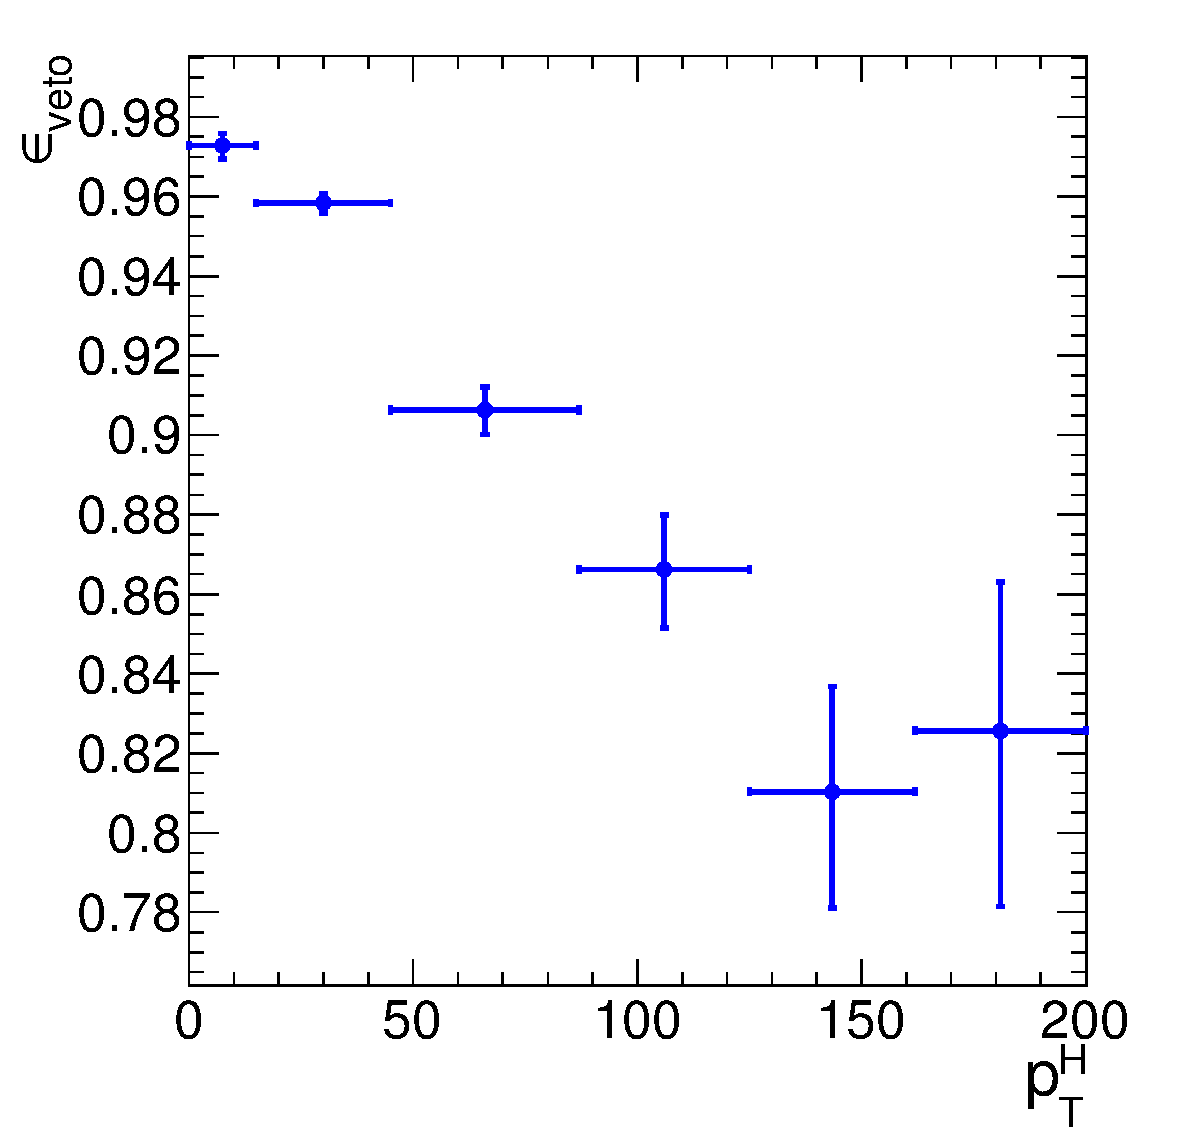
\includegraphics[width=0.5\textwidth]{images/eff_vs_pth.pdf}
\caption{Efficiency of the b-tagging veto in different bins of \pth.\label{fig:veto_eff_pth}}
\end{figure}
\begin{figure}[htb]
\centering
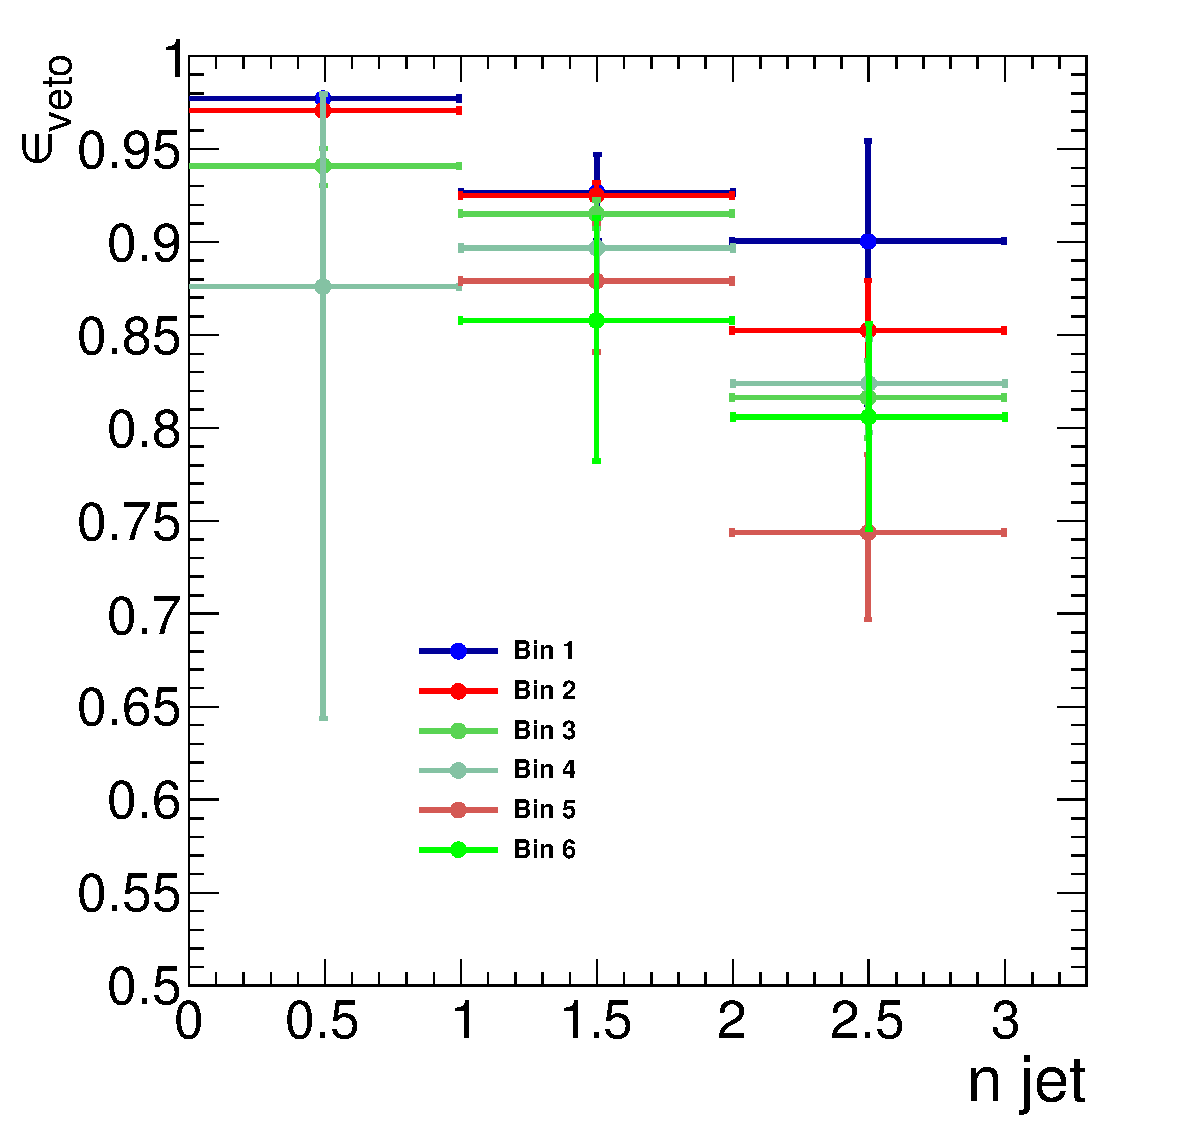
\includegraphics[width=0.5\textwidth]{images/eff_vs_jet.pdf}
\caption{Efficiency of the b-tagging veto in different bins of \pth, as a function of number of jets.\label{fig:veto_eff_njet}}
\end{figure}

The nuisance parameters reported in table \ref{table:jet_binning_theory} have then been calculated for each \pth bin embedding the veto efficiency and using the following formulas:
\begin{equation}
QCDscale\_ggH=\frac{ggH0*f_{0}*\epsilon_{0}+ggH1in0*f_{1}*\epsilon_{1}}{ggH0*f_{0}*\epsilon_{0}+ggH1in0*f_{1}*\epsilon_{0}}
\end{equation}
\begin{equation}
QCDscale\_ggH1in=\frac{ggH1in1*f_{1}*\epsilon_{1}+ggH2in1*f_{2}*\epsilon_{2}}{ggH1in1*f_{1}*\epsilon_{1}+ggH2in1*f_{2}*\epsilon_{1}}
\end{equation}
\begin{equation}
QCDscale\_ggH2in=1
\end{equation}

These nuisance parameters are expected to be equal to one in case the efficiency is independent on the number of jets, i.e if $\epsilon_0 = \epsilon_1 = \epsilon_2$.\\
The values obtained are reported in table \ref{table:jet_binning_meas} divided in bins of \pth.

\begin{table}[h]
\caption{Values of the jet binning nuisance parameters for different \pth bins.}
\label{table:jet_binning_meas}
\begin{center}
\begin{tabular}{ccccccc}
& Bin 1 & Bin 2 & Bin 3 & Bin 4  & Bin 5 & Bin 6\\
\hline
QCDscale\_ggH  & 0.998  &   0.993  &   0.989  &   1.000  &   1.000   &  1.000 \\
QCDscale\_ggH1in &0.997   &  0.993  &   0.984  &   0.975 &    0.946 &    0.974  \\
\end{tabular}
\end{center}
\end{table}

%Detailed summary of main sources of systematic uncertainty (normalization, experimental and theoretical)
% is presented at Table~\ref{tab:Systematics}.

%-------------------------------------------------------------------------------
\subsection{Monte Carlo statistics}
%-------------------------------------------------------------------------------

Due to the large range of weights to correct other MC pile up distribution to
match that in data, the effective size of the MC samples are sometimes smaller than
the actual number of events in the sample.
The statistical uncertainty of the event yields estimated from MC samples
is reflected in the final result.

%-------------------------------------------------------------------------------
\subsection{Treatment of systematics in the shape analysis}
%-------------------------------------------------------------------------------

One can distinguish between normalization uncertainties, where a systematic
effect is changing the normalization assuming the shape is not affected, and
shape uncertainties where the actual change in the shape of the distribution is
taken into account. The normalization uncertainties enter the shape analysis as
a constant normalization factor, whereas for shape uncertainties the nominal and
the $+1\sigma$ and $-1\sigma$ shapes enter the analysis in form of three histograms
with the same normalization. 

For the W+jets background, the shape differences for different jet \pt thresholds in the 
di-jet control sample are considered separately for electron and muon fakes, while the
other sources of systematics are taken as normalization uncertainties as in the cut-based
analysis.

Effects from experimental uncertainties are studied by applying a scaling and/or
smearing of certain variables of the physics objects, followed by a subsequent
recalculation of all the correlated variables. This is done for Monte Carlo
simulation, to account for possible systematic mismeasurements of the data.
All experimental sources from Section~\ref{subsec:expsyst} but luminosity
are treated both as normalization and shape uncertainties.
For background with a data-driven normalization estimation,
only the shape uncertainty is considered.

To account for statistical uncertainties, for each distribution going into the shape analysis, 
the $+1\sigma$ and $-1\sigma$ shapes were obtained by adding/subtracting the statistical error 
in each bin and renormalize it to the nominal distribution. In addition to this procedure a constant 
normalization uncertainty due to the finite statistics of the sample, used to extract the shape, is assigned.
